\documentclass{article}

\usepackage[utf8]{inputenc}
\usepackage{graphicx}
\usepackage{geometry}   \geometry{margin=1in}
\usepackage{amsmath}
\usepackage{xcolor}
\usepackage{float}
\usepackage{longtable}
\usepackage{multirow}
\usepackage{natbib}
\usepackage[nonumberlist]{glossaries}

\makeglossaries
\loadglsentries{glossary}


\title{Hot Swappable Pedalboard and Routing System:\\Progress Report 4}
\author{Nicholas Pham}
\date{February 2019}

\begin{document}

\maketitle
\begin{center}
    Electrical Engineering \\
    Scott Kuindersma, Jim MacAurthur
\end{center}

% \newpage
% \glsaddall
% \printglossaries
% \newpage


% \newpage
% \bibliographystyle{plain}
% \bibliography{ThesisSources}

% \section{Appendix}

\section{Prototype Measurement Methods}
	\subsection{Swap Time}
	The success of this project in terms of a solution for improving the process of auditioning guitar pedals will be mostly a result of this measurement: how much time is saved swapping between pedals when using this system compared to the standard manual method?  The experiment used to measure this difference should simulate the expected operating conditions of the system.  In this case, a participant will conduct two tasks, and the time required to complete each of these tasks will be recorded.  For both tasks, the user begins with a guitar with its output connected through a single guitar pedal.  They must safely remove this guitar pedal from the signal chain, set it down in a defined location, touch a second location, then re-insert the pedal back into the signal chain.

	The first task is the control.  The guitar pedal is connected in the standard way, with an instrument cable connected from the output of the guitar to the input of the pedal.  The output of the pedal is connected to the input of a guitar amplifier.  The pedal is powered with a standard 9VDC wall wart adapter.  See Figure \ref{fig:SwapTimeControlSetup} for a graphical representation.  The participant will be wearing the guitar (with a strap over their shoulder) to simulate real-world conditions.  To begin, the participant will have their left hand on the guitar's neck and their right hand touching the bridge (or the opposite in the case of a left-handed participant).  The pedal is set on a of standard height to mimic the environment of testing pedals in a guitar store, instead of on the floor.  After a countdown to let the participant know when to start, the timer will begin and the participant will quickly but accurately disconnect the pedal and place it on a marked rectangle on the table (shown in red).  The participant will, leaving the pedal in this marked rectangle, touch a second marker on the table (shown in blue).  This is to simulate the need to grab a second pedal without the experiment actually requiring the use of a second pedal.  After touching this blue marker, they will return the red rectangle to grab the pedal and re-insert it into the signal chain, making the input, output and power connections.  Then the participant will return their hands to the starting position on the guitar, which will signal the observer to stop the timer.  This measurement represents the time required to swap between pedals in the standard manual method.

	The second task is tests the hypothesis that the solution will decrease the swapping time.  This time the hot swapping unit is sitting on the table, with the instrument cable from the guitar plugged into its master input, and its master output connected to the input of a guitar amplifier.  The same pedal used for the control is connected to a plate (including all power and signal connections).  Before the task begins, this connected plate and pedal are inserted into one receiver on the hot swapping unit.  Again, the participant begins with their hands on the guitar.  When the timer starts, the participant removes the pedal and plate from the receiver, places it in the red rectangle, touches the blue marker, then retrieves the pedal and plate and reinserts it into the hot swap unit.  The timer stops when the participants hands both return to the guitar.  

	Both of these tasks should be repeated several of times for each participant, in this case three times, to ensure that a reliable measurement is recorded.  The test should also be performed with different pedals, especially ones of different size and with different I/O locations.  These pedals should be representative of the variety of pedals available.  The set of three pedals in Table \ref{tab:SwapTestPedals} should be representative of the range of products available that are compatible with the hot swapping system.  This means that each participant will perform nine trials of each task, totaling 18 trials.  Each trial should be no longer than one minute (and will likely be much less) so this is not an unreasonable number of tests per participant.  This experiment then should be conducted for a number of participants, at least ten, which should include both guitarists and non-guitarists alike.  Guitarists should have an easier time with the standard method, but comparing the measurements of non guitarists with guitarists should give an indication of how intuitive and simple the device is to use.  


	\begin{table}
	\begin{center}
	\begin{tabular}{ |c|p{8cm}| }
	\hline
	 Type Name & Description \\ 
	 \hline
	 $A$ & Mini sized pedal with side mounted jacks (similar to the TC Electronic Polytune 2) \\
	 $B$ & Standard sized pedal with top mounted jacks (similar to the EarthQuaker Devices Bit Commander) \\
	 $C$ & Oversizd pedal with side mounted jacks (similar to Electro Harmonix B9) \\
	 \hline
	\end{tabular}
	\caption{Set of three pedals used to represent the range of available products.}
	\label{tab:SwapTestPedals}
	\end{center}
	\end{table}

	Because this experiment requires some physical setup and scheduling for participants, it has not yet been conducted, but is planned for the week of February 18th after the PCBs are sent for fabrication.  For more details see the schedule near the end of this document.

	\subsection{Compatibility}
	The measurement for compatibility is not so much a matter of setting up a physical test but in determining which guitar pedals are likely to be available at music equipment retail locations and using the stated specifications for these to determine what ratio of them are compatible with the hot swapping device.  In this case, the list of common pedals was compiled by visiting brick and mortar music stores and taking stock of the products they had in stock.  Notably, the two Guitar Center locations in Boston were used to collect this data.  This list of available pedals which were photographed at the retail locations was entered into a spreadsheet.  Each entry was matched with a user manual and the available technical specifications were recorded.  These included:

	\begin{itemize}
		\item Physical Dimensions
		\item Range of Operating Voltages
		\item Required Current
		\item SNR
		\item Number and Description of I/O
		\item Input and Output Impedance
	\end{itemize}

	Data for more than 150 products from more than 25 companies were recorded.  This information was used to influence the design with the goal of accommodating the greatest number of available products.

	\subsection{Signal to Noise Ratio}
	The signal to noise ratio was measured for several different configurations of the unit.  An Audio Precision System One (AP) was used for all measurements.  This is a data acquisition device which can function as a test signal generator and a data recorder to measure the effect of the device under test.  The AP was connected to a computer via USB running its associated APWin software, allowing for control, processing, and visualization of the data.  For the SNR tests, one output of the AP was connected via a BNC-to-1/4" cable to the input of the device under test, and the output of the device under test was connected via a second BNC-to-1/4" cable to the corresponding input on the AP.  The AP's monitor output was connected to an oscilloscope to monitor the signal in real time.  To record the data, the AP measured the noise floor of the input and printed the value in dBu.  For each configuration being measured, the noise floor was captured for 20 trials.  The signal-to-noise ratio can then be computed from this noise floor measurement and the maximum supported signal for the device, which with a relay is almost arbitrarily large.

	The first test ($A$) was a control to understand the AP's own noise floor.  In this test, the output of the AP was connected directly to the input via a two foot BNC cable.  In this test, any noise recorded would be from the AP system itself, or noise picked up by this two foot coaxial cable, which limits the minimum detectable noise floor for the system under test.

	The second test ($B$) is of the prototype device with no power connected, and the signal switching relay on the receiver set to bypass.  Because the signal is mechanically connected directly from the input to output and no active circuitry is powered, this configuration should have the minimum noise floor among all measurements with the device under test.

	The third test ($C$) is of the prototype device with power connected and the signal switching relay on the receiver set to bypass.  In this case, the power supply is powering digital circuits on the same board as the analog signal, so a higher noise floor is expected.

	The fourth test ($D$) is of the prototype device with no power connected and the signal switching relay on the receiver set to send/receive.  In this case, a plate is inserted into the receiver with the plate's I/O connected to a guitar pedal which itself is in a hardwire bypass position, meaning that the plate's inputs and outputs are mechanically connected to each other.  This test will determine how much noise is picked up from the environment and the rest of the circuit board when the signal passes through the additional traces, pogo pins, cables, and jacks in the send/receive mode.

	These tests are summarized in Table \ref{tab:SNRtests}.

	\begin{table}
	\begin{center}
	\begin{tabular}{ |c p{8cm}| }
	\hline
	Test ID & Description \\ 
	\hline
	$A$ & Measure test system noise.  AP output connect to AP input via 2' BNC cable. \\
	$B$ & Measure relay noise.  No power.   AP output connected to device under test (DUT) input, DUT set to bypass, DUT output connected to AP input. \\
	$C$ & Measure power supply noise.  Power connected.  AP output connected to DUT input, DUT set to bypass, DUT output connected to AP input. \\
	$D$ & Measure operation nose.  Power connected.   AP output connected to DUT input, DUT set to send/receive, plate inserted with hardwire bypass connection, DUT output connected to AP input.\\
   	\hline
	\end{tabular}
	\caption{Summary of SNR testing.  The AP System One was used to measure THD+N.}
	\label{tab:SNRtests}
	\end{center}
	\end{table}



	\subsection{Frequency Response}
	The frequency response of the unit was measured with the same Audio Precision device and setup as the signal to noise ratio.  For this test, the AP output a sine wave sweep over a set frequency range and recorded the response of the device under test.  The sweep consisted of 51 discrete frequencies ranging logarithmically from 10Hz to 30kHz, which covers the entire audio range with some margin.  Though the requirement for flat frequency response was specified down to DC, it is not possible to test arbitrarily low frequencies, so 10Hz was chosen as a suitable minimum bandwidth.  These test sine waves were output at 0 dBu, which is equivalent to 0.775 VRMS or 2.19 Vpp.  The AP then recorded the amplitude of the returning sine wave.  This entire process was automated, with each discrete frequency being tested and measured several times, thereby producing a reliable result.  This test was conducted on all of the configurations described in the SNR measurement section.  

	\subsection{Switching Time}
	When the receiver switches between the bypassed signal and the processed signal from a pedal, the switching time refers to the period of downtime between when the bypassed signal is present on the output and when the processed signal is present.  In the case of this implementation, this is the time required for the blade of the relay to move from one contact to the other.  This test was conducted by setting the AP to output a sine wave at a low fixed frequency, and connecting a pedal set to attenuate the signal.  The AP output was connected to the input of the device under test, and the output of the device under test was connected to the input of an oscilloscope.  The oscilloscope's trigger was set to a level just less than the peak voltage of the input sine wave.  The test is conducted by first inserting the pedal into the receiver so that the output is an attenuated version of the sine wave which does not cross the trigger threshold.  Then the oscilloscope trigger is set to single mode so that the oscilloscope will capture and hold the signals in the time adjacent to when the trigger was activated.  When the pedal is removed from the receiver, the signal output switches from the attenuated version that was processed with the pedal to the bypassed sine wave at a great enough amplitude to trigger the oscilloscope.  With the oscilloscope stopped, the vertical bars were aligned with the discontinuities resulting from the relay blade being switched (it is floating in between the contacts), and these bars are used to measure the time the relay is floating.  The image of this transition along with the switching time measurement was saved from the oscilloscope to an image file.  The switching time test was performed five times.

\section{Prototype Measurement Analysis}
	\subsection{Swap Time}
	Though the swap time test has not been conducted yet, once the data is collected, a one tailed paired T-test can be used to determine if the hot swapping device fulfilled its order of magnitude improvement goal.  The paired samples correspond to one participant's time required to complete each of the two tasks outlined in the Methods section.  Because each participant will conduct multiple trials of both tests, they will contribute multiple paired samples to the T-test.  Because the possible values recorded are continuous and the paired measurements are relatively randomly sampled (by choice of participant), the T-test should be reliable.

	\subsection{Compatibility}
	The data collected was analyzed using MATLAB.  First, the data was broken down by company, and each company was assigned a numerical ID.  The number of pedals available from each manufacturer was counted.  Then the data was further broken down by pedal enclosure category.  Generally, each manufacturer will design many of their products to fit in the same enclosure, which keeps their procurement and design process simpler.  This allows the pedals to be grouped by enclosure type, meaning that all pedals offered with the same enclosure will have the same external dimensions and be mechanically compatible with the hot swapping device if any one of them is compatible.  Each enclosure type was also given an ID number, and was labeled with the company who uses it and the number of products being offered by that company using this enclosure type.  This data was plotted using a stacked bar graph as seen in Figure \ref{fig:pedalsAvailable}, with the company ID numbers listed in Table \ref{tab:pedal_companies}.  Note for instance that Company 12 (Boss) offers more than thirty pedals, and the vast majority of these use the same variety use the same type of enclosure, meaning that compatibility with this type of enclosure is a greater priority than a lesser used one, such as the type used by Company 9 (ProCo).  Note that the plot only shows effects with their physical dimensions listed in the manual, which explains why J Rockett Audio, which had two products, has no bar on the graph.

	\begin{figure}
		\centering
		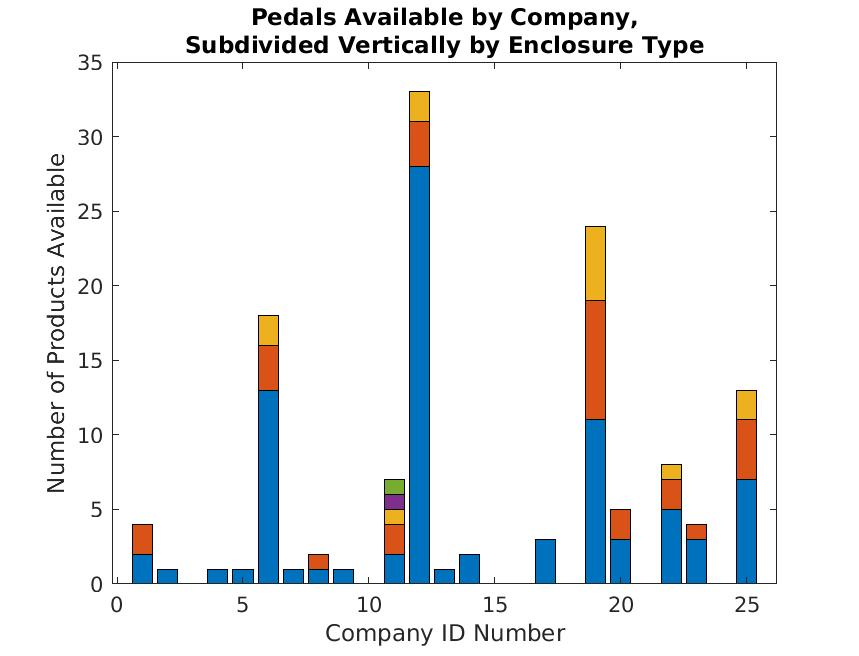
\includegraphics[width = 0.6\textwidth]{PR4Images/PedalsAvailable.jpg}
		\caption{Number of guitar pedals available by manufacturer ID.  The bars are divided vertically by the type of enclosure used, with the most popular enclosures on the bottom.}
		\label{fig:pedalsAvailable}
	\end{figure}


	\begin{table}
	\begin{center}
	\begin{tabular}{ |c c c| }
	\hline
	 Company Name & Company ID & Number of Products Available \\ 
	 \hline
	Seymour Duncan    &  1        &  4     \\
    BBE               &  2        &  1     \\
    J Rockett Audio   &  3        &  2     \\
    Tech 21           &  4        &  2     \\
    Ampeg             &  5        &  2     \\
    MXR               &  6        & 18     \\
    Korg              &  7        &  1     \\
    Fulltone          &  8        &  6     \\
    ProCo             &  9        &  1     \\
    Danelectro        & 10        &  3     \\
    Digitech          & 11        &  7     \\
    Boss              & 12        & 33     \\
    Eventide          & 13        &  1     \\
    Way Huge          & 14        &  2     \\
    Egnater           & 15        &  1     \\
    Line6             & 16        &  1     \\
    Fender            & 17        &  3     \\
    Voodoo Lab        & 18        &  1     \\
    EHX               & 19        & 26     \\
    Ibanez            & 20        &  5	   \\    
    Maxon             & 21        &  1     \\
    EarthQuaker       & 22        &  8     \\
    JHS               & 23        &  4     \\
    Keeley            & 24        &  5     \\
    TC Electronic     & 25        & 13     \\
   	\hline
	\end{tabular}
	\caption{List of guitar effects manufacturers and their associated ID numbers.}
	\label{tab:pedal_companies}
	\end{center}
	\end{table}

	To determine which pedals will be mechanically compatible, their dimensions were compared with the dimensions of the currently plate.  Because of the "opposite corners" mechanical connection technique where the screws from two of the pedal's corners are connected through the plate to make the mechanical connection, any pedal will fit if the distance between its opposite corners (less some factor to account for the positioning of the screws slightly inside the outer dimensions of the enclosure) is within the range permitted by the plate design.  The plate prototype can support pedals with a minimum screw hole distance of 2.5" and a maximum distance of 5.2".  Figure \ref{fig:pedalcompatibility} describes the compatibility of the plate prototype with the different pedals available.  The x axis represents the distance between opposite screw holes for a given enclosure.  The data points of the scatter plot represent each type of enclosure cataloged, positioned by this screw hole distance and by the number of different products available that use this same enclosure, which is shown on the left y axis. The line plot is the cumulative ratio of the products available with their screw hole distance less than the current $d$ value on the x axis out of the total number of pedals available.  Assume the plate can support all pedals up to a given dimension, this line can be used to determine the ratio of compatibility for the design.  The 80\% and 95\% goals are shown as horizontal lines.  The compatibility of the first prototype is depicted by the blue shaded region at left, which covers all screw hole distances up to 5.2".  The intersection of the rightmost boundary of this blue region with the line plot gives the current compatibility, which is just shy of 70\%.

	\begin{figure}
		\centering
		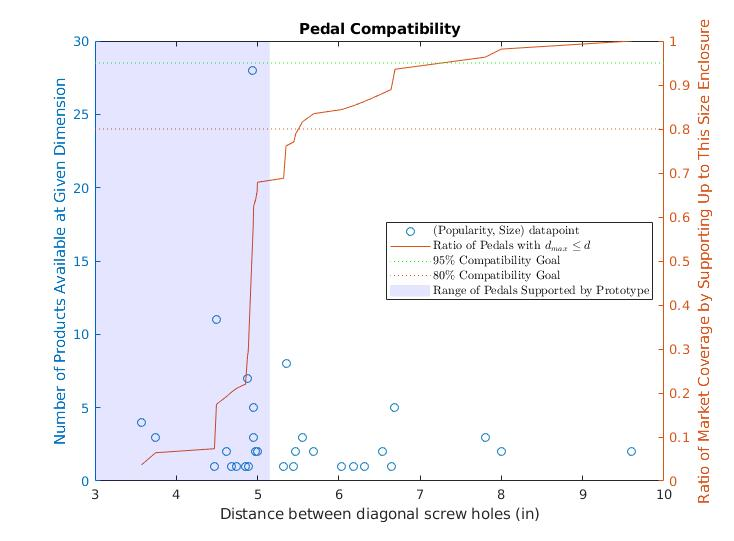
\includegraphics[width = \textwidth]{PR4Images/PEdalCompatibility.jpg}
		\caption{}
		\label{fig:pedalcompatibility}
	\end{figure}

	This plot can be used to improve the design of the plate to find a balance between increasing the size of the plate to improve compatibility while not wasting space.  For instance, there are two clusters in the x direction of pedals with screw hole distances less than 6" and 7", respectively.  Increasing the size of the plate to 6" would result in an 85\% compatibility ratio, which would meet the specifications.  This is a good trade-off of size versus compatibility.  In fact, increasing the plate size to 7" would allow the design to reach the 95\% goal.  However, if the plate size was increased enough to reach every single enclosure, the additional size would not add very much compatibility, so that would be a poor trade-off.

	Although the current prototype fails to meet either the 80\% or 95\% requirement, this is not a major issue.  The goal of the prototype was to test the hot-swapping features and get a sense for problems the plate might have.  With this groundwork in place, the plate size can be changed to fit requirements without much issue.

	COME BACK FOR POWER, I/O Considerations

	\subsection{Signal to Noise Ratio}
	The data collected from the measurements is summarized in Table \ref{tab:SNRresults}.  Test $A$ shows the limits of observation with the Audio Precision measurement device.  Because the system has -107 dBu noise floor by itself, it will not be able to detect if the DUT has a lower noise floor.  This is an industry standard measurement device, so using this instead of a potentially lower noise one is reasonable.  In addition, the actual values obtained during this tests qualitatively seemed affected by quantization noise.  Only a handful of discrete values were recorded over the 20 trials for this test.  These measurements taken were of the noise floor, which is only one of the two values needed to compute the SNR.  The maximum signal level is also required.  This can be difficult to determine when relays are used, as the signal can be arbitrarily large up to the maximum isolation voltage of the relay, which could be in the 100s or 1000s of volts, which would skew the SNR.  A better value to use would be the maximum supply voltage the device makes available to pedals, 18V, as this is the largest expected signal for the receiver under normal circumstances.  In units of dBu, 18Vpp = 12.7279Vrms = 24.3136dBu.  Therefore, the SNR of the system is the absolute value of the mean measured THD+N value plus 24.3136.  These SNR values are also given in Table \ref{tab:SNRresults}

	Test $B$ shows the noise floor for the device with no power connected.  The mean noise was the same as test $A$, which shows that the relay is an excellent choice for signal integrity.

	Test $C$ shows the noise floor with the power connected.  Here the mean noise floor increased to -82 dBu, a three order of magnitude increase.  This is a result of the switching noise from the switching power supply being coupled onto the audio signal.  This noise is particularly problematic because it had a noticeable frequency component around 20kHz, which is just at the upper end of the audio spectrum, meaning that this noise could be heard through the speakers during use.  Although the resulting SNR does meet the 90dBu minimum requirement, it does not achieve the desired 120dBu requirement.  Therefore, effort should be taken to mitigate the resulting power supply noise.

	One simple solution for the power supply noise issue is the introduction of a common mode choke at the power input to the device.  The common mode choke performs a similar function to a pair of inductors connected in series with the power and ground lines respectively.  By limiting the change in current on these wires, the choke can reduce switching noise, even noise that is present on the system's ground.  To this end, an additional test $C'$ was performed with a choke connected between the switching power supply and the device's power input.  As can be seen, the noise floor reduced markedly, returning to near the limits of the AP measurements system.  

	Because the previous test successfully demonstrated the effectiveness of the choke in mitigating the power supply switching noise, the remaining test was modified to include the common mode choke, now labeled as test $D'$. The noise floor increased slightly over the bypassed mode, which makes sense as the audio signal now must travel through additional traces, wires, and components.  In addition, the guitar pedal power supply is also traveling through additional unshielded cables, all of which provides opportunity to pick up noise.  However, the noise floor is still very low, and meets the 120dBu requirement.  With the inclusion of the common mode choke, no changes must be made on this system to maintain the specified requirements.

	\begin{table}
	\begin{center}
	\begin{tabular}{ |c c c c| }
	\hline
	Test & Mean THD+N (dBu) & Variance (dBu) & SNR (dBu) \\ 
	 \hline
	$A$ & -106.9621   & 0.0178 	& 131.2757 \\
	$B$ & -106.8596   & 0.0157 	& 131.1732 \\
	$C$ &  -82.0101   & 0.1373  & 106.3237 \\
	$C'$ & -106.6603   & 0.1566 & 130.9740 \\
	$D'$ & -104.9962   & 0.0357 &  129.3098 \\
   	\hline
	\end{tabular}
	\caption{Results of SNR testing.  The AP System One was used to measure THD+N.}
	\label{tab:SNRresults}
	\end{center}
	\end{table}

	\subsection{Frequency Response}
	The frequency response measurement recorded data at 51 different frequencies, ranging logarithmically from 10Hz to 30kHz.  At each frequency, the AP sent a 0dBu sinusoid and measured the amplitude of the signal returned at its input.  The frequency response was measured with the hot swapping device in send/receive mode with the common mode choke in place to replicate expected operating conditions.

	\subsection{Switching Time}
	\subsection{Transient}



\section{Full System Implementation}
	With verification of the prototype complete, the implementation of the full system can move forward.  The full system will contain:

	\begin{itemize}
		\item (6) receiver units
		\item (4) 2x2 analog multiplexer for signal routing
		\item User Interface
		\item Power supplies for the above components
	\end{itemize}

	Because of the necessity to order PCBs in quantity, it is beneficial to design the system in a modular fashion such that several boards can be used to construct the entire system.  This is a feasible goal because of the system topology.  In addition, during the design phase for the prototype components were selected to allow for two receivers per board.  In particular, these include the LV8548MC dual H-bridge driver, and the ATTiny40 microcontroller, which was selected to provide enough GPIOs to control two receivers.  With this in mind, the additional signal routing and user interface components can be integrated locally on each of the boards.

	INSERT FIGURE DEMONSTRATING THE MODULARITY

	This method would also allow a larger system to be constructed simply by connecting more of these modular boards (and increasing the maximum supply current of the power supply).  The following sections will detail the changes made to the prototype designs to accommodate this, as well as the new designs for the analog signal routing and user interface.

	\subsection{Microcontroller Selection}

	Though the prototype was initially designed for easy integration of the additional routing and user interface subsystems, the ATTiny40 is not adequate to support these.  The main issue with the ATTiny40 is its limited GPIO count.  In addition to the 16 pins required for the two receivers, fourteen pins must be allocated for the user interface and eight for the routing on each module.  This totals to 38, the minimum requirement for GPIO pins.  Extra pins for serial communications, debugging, and future potential connections should be included as well. 

	Another issue with the ATTiny40 was its lack of on-chip debugging capability.  Because of the device's focus on a limited feature set, it's proprietary TPI (Tiny Programming Interface) for programming did not support on-chip debugging via JTAG or similar \cite{ATTiny40_datasheet}.  However, the programming interface should be compatible with Atmel's ICE in-system programmer which had already been purchased for use with the ATTiny40.  Other desirable features include an on-board oscillator to drive the clock for applications such as this that do not require a highly accurate clock, and 5V compatibility to interface easily with the existing system, most notably the relays.  This will reduce the number of external components necessary, minimizing cost and complexity.

	With these requirements, the ATMEGA3209-AFR was selected as the best option.  At \$1.47 a piece \cite{ATMEGA3209_digikey}, the device is not quite as cheap as the PIC16F15385 (\$1.25 a piece) \cite{PIC16F_datasheet}, but it uses the same development tool chain as the ATTiny40 from before, which will make the switch of devices easier.  In a hand-solderable 48-TQFP package, this chip comes with 41 GPIO each capable of generating an interrupt, an internal 20 MHz oscillator, and a one-wire Unified Program Debug Interface (UPDI) which, as the name suggests, allows for in-system programming and debugging \cite{ATMEGA3209_datasheet}.

	\subsection{Receiver Subsystems}

	Adapting the receiver from the prototype into the module is fairly straightforward as a result of the prototype's success.  Each of the two receivers on board a single module has the same LM317 programmable voltage regulator set up as before.  The two receivers will share one LV8548MC dual H-bridge driver, which is driven by the ATMEGA3209.

	One major difference in the implementation is the mechanical configuration of the pogo-pins.  Because the pogo-pins were directly connected to the board on the prototype, much of the board area was wasted, with a major fraction of the surface devoted to the mechanical alignment of these electrodes.  This issue is even more important when designing the two-receiver module, as now the pins must be aligned for each of the receivers, meaning that the separation between the pins and hence the length of the circuit board must be no shorter than the height of one receiver (see Figure \ref{fig:module_mech_layout}).  To be more space efficient, the module will consist of a main board with all of the devices along with several remote boards connected via board-to-board connectors for the pogo-pins and user interface.  This will allow the mechanical placement of the main board to be independent (relatively) of the pogo-pins.  This will also reduce the vibrations and shocks to the main board as a result of the pogo-pins being depressed and released.

	\subsection{Analog Signal Routing}

	Each module will contain a two input, two output mixer.  Each of the two outputs 1 and 2 can be connected to either input $A$ or $B$, as well as the sum of the two inputs $A + B$.  Table \ref{tab:routing_outputs} shows the possible outputs.  As can be seen, there are only signals that must be available for the output.

	\begin{table}
	\begin{center}
	\begin{tabular}{ |c|c c| }
	\hline
	 Permutation & Output 1 & Output 2 \\ 
	 \hline
	 1 	& $A$ 	& $A$ \\  
	 2 	& $A$ 	& $B$ \\
	 3	& $A$ 	& $A+B$ \\
	 4	& $B$ 	& $A$ \\
	 5	& $B$ 	& $B$ \\
	 6	& $B$ 	& $A+B$ \\
	 7	& $A+B$ & $A$ \\
	 8	& $A+B$ & $B$ \\
	 9	& $A+B$ & $A+B$ \\
	 \hline
	\end{tabular}
	\caption{List of the $2^3$ possible output signals for each routing module.}
	\label{tab:routing_outputs}
	\end{center}
	\end{table}

	With this in mind, the specific implementation of the routing mechanism can be designed.  For the same reasons that relays were chosen to actuate the signal switching in the receiver subsystem, they should also be used here.  This is essential especially when an output is connected directly to an input, such as permutation 2 in Table \ref{tab:routing_outputs}, which will preserve both the SNR and frequency content of the signals in addition to the signal's output impedance.  However, when a summed output is chosen ($A+B$), the signals must necessarily pass through a summing amplifier, which will result in a low impedance output.  In this instance, the use of a mechanical relay is not strictly necessary.

	The specific implementation of the routing subsystem is shown in Figure \ref{fig:routing_schem}.  Each output selector is in essence a three-to-one multiplexer.  The requirement for mechanical relays when the sum output is not selected requires the use of mechanical relays throughout, as each can only switch between two inputs.  Thus, each three-to-one multiplexer includes two of the same DPDT relays used for the receivers despite not all of the throws being in use, as they were cheaper than any SPDT relay.  Using the same EA2-5SNJ relays also minimizes additional components on the BOM.  The use of latching relays here is even more beneficial than in the receiver, as these relays will likely be set in a position for long periods of time, so the reduced current and heat dissipation compared to a non-latching relay is very beneficial.

	To generate the summed $A+B$ signal, a standard inverted summing amplifier is used.  The resistors were chosen to each be $10K\Omega$ so that each input is at unity gain.  Higher resistor values were avoided to reduce thermal noise.  However, the input impedance to the inverted amplifier is just the value of the input resistance, so non-inverting op-amp buffers are required to prevent preceding circuits on $A$ and $B$ from interacting with the summing amplifier.  As this already requires three op-amps and the output signal would be inverted, an additional unity gain inverted buffer is used at the output to re-invert the signal, resulting in $A+B$.

	This summing amplifier and related circuitry requires its own analog supply voltage.  In the worst case, the maximum voltage swing of each input signal $A$ and $B$ should be no more than 18Vpp, which is the maximum supply voltage available to a pedal from a receiver.  This means that the summing amplifier should ideally be able to swing 36Vpp.  However, the power supply currently being used provides 24VDC.  This means that without modification, the summing amplifier will not be able to sum all possible signals without clipping.

	There are several possible solutions to this issue.  One would be to change the device's power supply.  Moving to a chassis mount 48V supply like Mean Well's LRS-150-48 \cite{datasheet:LRS-150-48} (\$22.50 from Digikey \cite{Digikey:LRS-150-48}) would allow for plenty of headroom and could provide much more current (in this case 3.3A), enough for six pedals each drawing 500 mA while leaving some budget for the device's own circuits.  A new power supply could be chosen to avoid the issue of switching noise in the audio range; the switching frequency of the LRS-150-48 is 65kHz, well above the audio spectrum.  Linear regulators could be used to drop the input voltage to the desired level, in this case just above 36V.  This supply could then be split with a resistive divider to provide the virtual ground needed for the op amp summer.  However, a chassis mount supply would involve introducing 120VAC wall voltages into the unit, which would not satisfy the SELV compliance specification.  Brick-type supplies in this voltage and current range are prohibitively expensive, such as the PSA120U-480L6 from Philhong USA for \$38 \cite{Digikey:PSA120U-480L6}.

	A second option would be designing an on-board boost-buck converter to create the desired supply voltages.  In this case, this switching supply could be used to generate an arbitrary voltage, so a bipolar 18V or 24V set of rails could be created.  This would allow for sufficient headroom for the summing amplifier, and by virtue of the bipolar supply would not require AC coupling the summed signals to a virtual ground: they could remain DC coupled.  A switching supply would also be more efficient than a linear regulator.  However, the added complexity of implementing a switching voltage regulator, is probably not worth the benefits.  Noise from the on-board supply would need to be carefully controlled so as to avoid corrupting the audio signals.  In addition, a linear regulator would likely still be used to really clean up the residual ripple from a switching regulator.

	The third option is simply using a linear regulator to even out the current 24V supply and allowing the summing amplifier to clip at a lower voltage.  This is not as big an issue as it seems at first.  Though the worst case scenario is two 18Vpp signals being summed in phase, this would require the user to be using two pedals in 18V mode at full output level.  The more likely use case with two 9V pedals would work fine with the 24V supply.  If the user does cause the summing amplifier to clip, they can simply reduce the output level of the two pedals.  In addition, if the amplifier were able to sum two outputs to 36Vpp, this would cause the next pedal in the chain to clip as well because of its voltage could be 18V at maximum, so the 36Vpp output would only be usable at the input of the amplifier where it would not clip the amplifier input.  This is also the simplest option, as it requires only a linear regulator to clean up the 24V input and a resistive divider to generate the virtual ground reference voltage.  

	INSERT TABLE COMPARING PROS AND CONS OF THE POWER SUPPLY OPTIONS

	Because of the simplicity of the third option and its relatively limited negative effects, this method was chosen to provide the supply for the summing amplifier.  To maximize the dynamic range of the summing amplifier, the regulated supply rail should be as close as possible to the 24V input.  The 200mV noise spec on the power supply means that the regulator must drop at least 200mV.  An adjustable regulator would be useful here to precisely set the output voltage.  The LM317 adjustable regulator used for the receiver is one option.  However, it's minimum 3V drop between input and output means that the analog supply rail cannot be set any higher than 21V \cite{atasheet:LM317}.  This decreased headroom is not desirable, so a lower dropout device would be preferable.

	Although the LM317 is billed specially as an adjustable regulator, most fixed voltage regulators can also be used in an adjustable mode in a similar configuration.  This is noted in the LM7805 datasheet, which shows in Figure 3 how the fixed voltage across the output and common terminals can be used to set the current through a second resistor between the common terminal and ground, much like the LM317 application \cite{datasheet:LM7805}.

	FINISH DESIGN OF REGULATOR CIRCUIT

	From this analog supply voltage, a virtual ground can be produced from a simple resistive divider circuit.  Though in theory this is susceptible to sagging due to large current loads, this should not be an issue for this application because the reference voltage is connected only to the inputs of two op-amps, and tied to the audio signal through large resistors.

	ADD SCHEMATIC AND MATH TO SHOW THAT LITTLE SAG WILL OCCUR

	The $A$ and $B$ inputs are each connected through a decoupling capacitor to their respective op-amp buffer inputs, and are pulled to the reference voltage via 1M resistors.  The 2.2M resistors were chosen to prevent the $A$ and $B$ signals from being heavily loaded down.  In the worst case, a signal could pass by six of these buffers, as show in Figure \ref{fig:worstcaserouting} without being buffered, so the equivalent resistance of six of these pull-up resistors must not be too low.  The equivalent resistance of six resistors in parallel is

	$$ R_{eq} = \frac{1}{\sum\limits_{i=1}^{6}\frac{1}{R}} = \frac{R}{6} $$

	INSERT FIGURE SHOWING WORST CASE ROUTING FOR LOADING

	so for 2.2M this is 367k$\Omega$.  Assuming a 10K$\Omega$ purely resistive output impedance from the guitar's pickups (on the high side for DC resistance but fairly reasonable for AC impedance), the input impedance should not be a major issue.  A large resistor value here also means the capacitance of the decoupling capacitor can be less to maintain a similar cutoff frequency, and it will be cheaper to have a higher quality plastic film or C0G ceramic capacitor in a smaller value.  The limit to choosing a very large resistor is the thermal noise, which may become a concern even with this value.  If this becomes an issue, the values can be adjusted once the board has been fabricated.  The cutoff frequency for the high pass filter formed by pull-up resistor and the decoupling capacitor should have its cutoff frequency on the order of 5-10Hz so it will pass the full audio range.  For a 2.2M resistor, this means

	$$ C = \frac{1}{2\pi R F_c} = \frac{1}{2\pi (2.2 \text{M}\Omega) (10 \text{Hz})} = 7.2 \text{nF}$$

	Because this is on the high end of the frequency range, the next larger standard value capacitor, 0.01uF, is used.  Kemet offers a 0.01uF film capacitor in through hole mounting for just \$0.25.  The film capacitors are more linear and have lower ESR and self inductance than typical ceramic caps, making them suitable for audio signal path usage.  The resistors can be standard.

	The op-amp selected should have low noise, low input bias current to prevent loading the input signal lines, and a rail-to-rail output to maximize headroom.  For op-amps compatible with a supply of 24V or more, Texas Instrument's OPA1679IDR is a good candidate.  At \$1.20 from Digikey, it is not cheap, but its datasheet claims 0.0001\% THD+N, a 10 pA max input bias current, and voltage output within 800mV of each rail \cite{datasheet:OPA1679IDR}.  These specs compare admirably to the TLV4172IDR and OPA4172IDR, each of which are twice the price.  Because there are not too many components in the audio path and its value as a reliable reference is paramount, it is appropriate to use more expensive and higher quality parts here.

	\subsection{User Interface}

	The above analog signal routing subsystem needs to be controlled by the user.  Because this device is designed to simplify the user experience, the user interface should be intuitive to use; no or few instructions should be needed to operate it.  The user interface should clearly indicate the current state of the signal routing, and the method by which the user can change the routing should be likewise linked to the physical signal connections being made.  To avoid disrupting the user from their focus on audio, the interface should be primarily visual and tactile in nature, as opposed to auditory.  For these reasons, the indication and actuation elements should be meshed, taking the form of push buttons with an integrated light.

	As described in Table \ref{tab:routing_outputs} above, each of the two inputs can be connected to each of the two outputs.  This includes cases where both inputs are connected to one or both of the outputs.  In no scenario can an output be connected to no input, which means that the user will never experience any "dead spots" where no sound can be heard.

	Qualitative tests were used to determine the effectiveness of such an indicator light.  An 8" $\times$ 1/2" $\times$ 1/4" clear acrylic sheet was cut using a laser cutter.  One side of this sheet was engraved with the same laser cutter in a continuous pattern to provide a rough surface off which light can reflect and refract.  A white LED was lit and place on one end of the sheet, facing the 1/2" $\times$ 1/4" rectangular side.  When the LED was held within 5mm or so of the face, the acrylic appeared to illuminate when viewing either of the 8" $\times$ 1/2" faces.  This rapid prototyping was conducted in a brightly lit machine shop, with lighting conditions similar to that expected in a guitar retail store.

	INCLUDE UI SKETCH SIDE VIEW

	Though specific mechanical design for this switch, as with the rest of the completed unit is not yet complete, the basic design is shown in Figure \ref{fig:UIsketch}.  As with the rapid prototype test described above, the central component of the subsystem is a beam made of clear 1/4" acrylic with the bottom side textured via laser cutter.  This beam functions as the light pipe used to direct and then scatter light from an LED, converting this light from a single source to an illuminated shape.  A white LED is inserted in a hole drilled on the smallest face of the beam, pointing down the length of the beam.  This hole should be centered on the face and is 3mm in diameter to fit a 3mm diameter LED.  The LED is connected via a twisted pair of wires to the main PCB (not shown), where it is powered by a constant current source.

	As mentioned, the acrylic beam's bottom is textured to allow the light from the LED to reflect and refract.  The acrylic rests on a longer aluminum beam for added support.  Between these is a thin layer of white vinyl or paper attached by pressure-sensitive adhesive to visually isolate the acrylic light from the underlying support structure.  Under one end of the acrylic, the aluminum beam sits on a limit switch actuator, which is used to detect when the user has depressed the acrylic beam.  On the opposite end, the aluminum extends beyond the extent of the acrylic.  The aluminum beam is pivoted on this end via a through hole.  This system is more clearly described in the force body diagram in Figure \ref{fig:UIFBD}.

	\subsubsection{User Interface Force-Body-Diagram and Switch Selection}

	INCLUDE UI FBD

	As can be seen, designing the system is simply a matter of balancing the torques on the beam.  Assuming no deflection of the beam, which is reasonable given the small magnitude of the forces and distances involved compared to the rigidity of the aluminum and even acrylic, and no friction, the system can be described in a static, undisturbed state by

	$$ F_{limit} l \ge F_{g_{AL}} \frac{l}{2} + F_{g_{acrylic}} \left( l - \frac{d_{max}}{2} \right) $$

	This requires that the torque produced by the operation force of the limit switch is greater than the torque produced by the weight of the beam.  Assuming an 8" $\times$ 1/2" $\times$ 1/4" piece of aluminum (this is on the larger side, which will give some margin for the limit switch force requirement), and the density of aluminum 2.7 g/cm$^3$ \cite{SolidsDensities}, 

	$$ F_{g_{AL}} = m_{AL}g = \left(16.39\text{cm}^3\right) \left(2.7 \text{g/cm}^3 \right) \left( 10^{-3}\text{kg}/\text{g} \right) \left( 9.8 \text{m/s}^2 \right) = 0.43 \text{N} $$

	A 6" $\times$ 1/2" $\times$ 1/4" (again also on the larger side) piece of acrylic with density 1.2 g/cm$^3$ \cite{SolidsDensities} would have weight

	$$ F_{g_{acrylic}} = m_{acrylic}g = \left( 12.29\text{cm}^3 \right) \left( 1.2 \text{g/cm}^3 \right) \left( 10^{-3}\text{kg}/\text{g} \right) \left( 9.8 \text{m/s}^2 \right) = 0.14\text{N}$$

	This means that the minimum required normal force by the limit switch before it activates is

	$$ F_\text{sw} \ge \frac{(l/2)0.43\text{N} + (l-d_\text{max}/2) 0.14\text{N}}{l} $$

	and is dependent on the specific geometry of the lever.  An upper bound can be found by substituting $l$ for all of the distances, which means that the operating force of the limit switch must be greater than the sum of the weights of the acrylic and aluminum, so $F_\text{sw} \ge 0.57\text{N}$, though something a little higher like 1N might be a good lower bound for the switch operating force to leave some margin.  On Digikey, switches' operating force is given in units of gram-force $gf$ where $1gf = 0.00980665\text{N}$ so this lower bound of 1N = $101gf$.

	The upper bound for the switch operating force is limited by the force required to depress the switch by the user when they press closest to the pivot, or at distance $d_\text{max}$ from the end of the lever furthest from the pivot.  Again this is dependent on the relative lengths and geometry of the design.  Keeping the acrylic beam as short as possible will reduce the difference in force required to activate the switch along its length.  As with the rest of this mechanical system, more work will be done once the PCB design has been sent out for manufacturing.  Because this design does not need to be completed before the PCB is designed and manufactured, this does not pose an issue with the timing of the project.

	\subsubsection{Button Layout}

	With these unified indicator-buttons, the remaining design for the user interface is the exact layout of the buttons.  As mentioned, they should be physically intuitive for the user to select the active inputs for each output.  The physically layout of the receivers is on a $3 \times 2$ grid.  The signal routing subsystems are used to connect the paired receivers on adjacent columns.  Figure \ref{fig:OverallUILayout} shows the overall layout of the receivers and the buttons.

	\begin{figure}
		\centering
		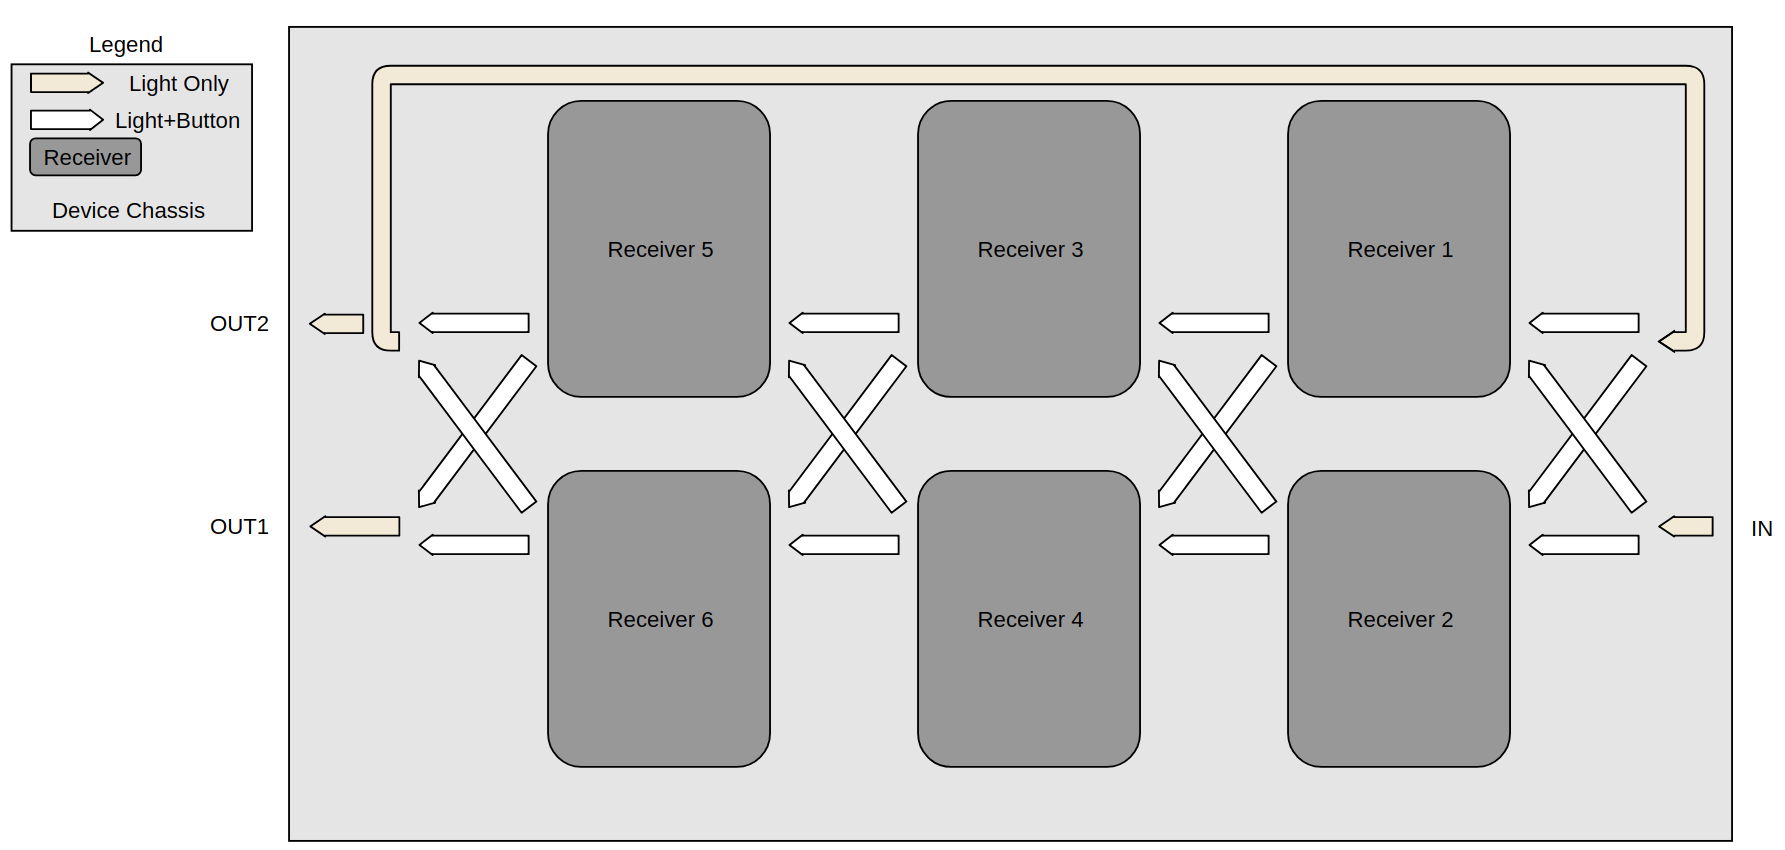
\includegraphics[width = \textwidth]{PR4Images/UIOverview.png}
		\caption{Overview of the user interface for understanding the physical layout of the overall unit.}
		\label{fig:OverallUILayout}
	\end{figure}

	To conform with guitar effects industry standards, the signal flow for the overall unit is from right to left.  Between each vertical pair of receivers (such as Receivers 1 and 2 in Figure \ref{fig:OverallUILayout} is a set of four integrated buttons and indicators, shown as white arrows.  Each set of these white arrows is connected to one module board and the board's routing subsystem.  Each button in the set is related to one particular signal routing direction.  For example, the arrow that points left from Receiver 2 to Receiver 4 indicates if the output of Receiver 2 is available on the input of Receiver 4.  In this example, that indicator would be lit if Receiver 4's input was either the output of Receiver 2 or the sum of the outputs of Receiver 1 and Receiver 2.  Each arrow shaped button toggles the state of both its LED and the relays associated with its connection.  In addition, there are a few lights, shown as tan arrows, that do not function as switches, and are lit depending on certain parameters.  For example, the indicators for IN, OUT1, and OUT2 are lit when a cable is plugged into the respective output to show that the connection has been correctly made.  In normal operation at a music store, the output will remain plugged in, so this will function as a de facto ON/OFF indicator.  The large indicator representing the feedback path will be turned on only when the feedback path is active: at least one of the two white arrows on the far right that point from the end of the feedback indicator into Receiver 1 and Receiver 2 are lit.

	\subsubsection{Control Finite State Machine}

	Each routing subsystem is a two input, two output mixer.  Each of the outputs can be the connected to either input or the sum of the inputs.  This means that these outputs can be controlled independently, so each set of white arrows can be split into two groups based on the output they control.  For instance, in Figure \ref{fig:UIarrowlabels}, buttons $a$ and $b$ control the top output while $c$ and $d$ control the bottom output.

	\begin{figure}
		\centering
		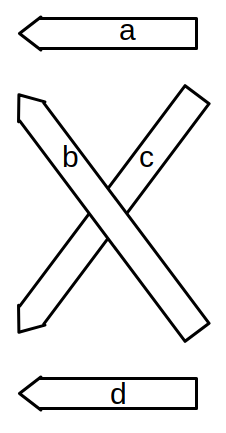
\includegraphics[width = 0.15\textwidth]{PR4Images/UIarrowlabels.png}
		\caption{Set of button-indicators.  These are associated with one module and are used to control the module's signal routing subsystem.  The letters are used for identification in this document.}
		\label{fig:UIarrowlabels}
	\end{figure}

	The switch logic and debouncing will be computed on the microcontroller.  The finite state machine depicted in Figure \ref{fig:UIFSM} will run in two instantiations on the microcontroller to cover the $a$ and $b$ set of switches along with the $c$ and $d$ set.  This diagram illustrates only the machine associated with the $a$ and $b$ switches.  This is Moore state machine where the output is determined by the current state.  The output/state is written in the boxes, and is described by STATE[1:0] where the bit 1 is the state of indicator $a$ and bit 0 is the state of indicator $b$.  The input vector is INPUT[1:0] where bits 1 and 0 represent whether switches $a$ and $b$ are asserted at any given time.

	\begin{figure}
		\centering
		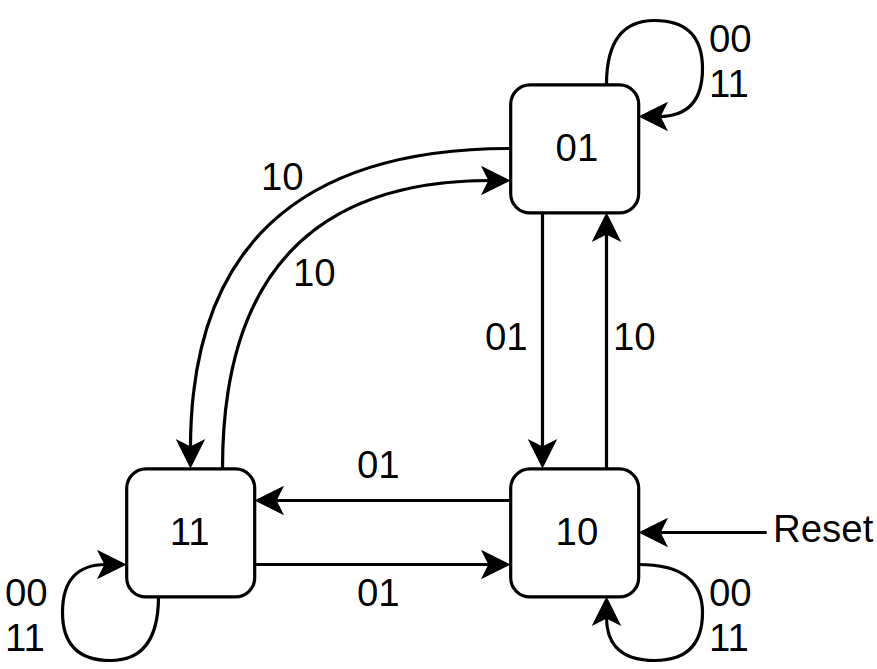
\includegraphics[width = 0.5\textwidth]{PR4Images/UIFSM.png}
		\caption{Finite State Machine describing the operation of the user interface for the signal routing.}
		\label{fig:UIFSM}
	\end{figure}

	As can be seen, the machine always starts in state $\mathtt{10}$, which means that the top input is connected to the top output in a "straight" line.  In terms of Figure \ref{fig:OverallUILayout}, this means that the unit will route the signal

	$$ \text{RECEIVER 1} \rightarrow \text{RECEIVER 3} \rightarrow \text{RECEIVER 5} $$

	This diagram does not indicate any information about the state of the relays in the actual signal routing subsystem.  This is because each FSM state, which is nominally tied to the LED state, also has a dedicated setting for those relays.  All of this information is summarized in a state transition table shown in Table \ref{tab:FSMtransistions}.  Note that state $\mathtt{00}$ should never be reached, as this would indicate that no output is currently selected.  If this state does mistakenly appear, it should transition to state $\mathtt{10}$, which is the default starting state.

	\begin{table}
	\begin{center}
	\begin{tabular}{ |c c|c c|c c|c c|}
	\hline
	\multicolumn{2}{|c|}{State/LED State} & \multicolumn{2}{|c|}{Relay Position} & \multicolumn{2}{|c|}{Input} & \multicolumn{2}{|c|}{Next State} \\
	\hline
	$a(d)$ & $b(c)$ & K1(K4) & K2(K3) & $a(d)$ & $b(c)$ & $a(d)$ & $b(c)$ \\
	\hline
	0 & 0 & 0 & 0 & X & X & 0 & 1 \\
	\hline
	\multirow{3}*{0} 	& \multirow{3}*{1} 	& \multirow{3}*{0} 	& \multirow{3}*{1} 	& 0 & 0 & 1 & 0 \\
						& 					&					&					& 0 & 1 & 1 & 0 \\
						& 					&					&					& 1 & 0 & 1 & 1 \\
						& 					&					&					& 1 & 1 & 0 & 1 \\
	\hline
	\multirow{3}*{1} 	& \multirow{3}*{0} 	& \multirow{3}*{0} 	& \multirow{3}*{0} 	& 0 & 0 & 1 & 0 \\
						& 					&					&					& 0 & 1 & 1 & 1 \\
						& 					&					&					& 1 & 0 & 0 & 1 \\
						& 					&					&					& 1 & 1 & 1 & 0 \\
	\hline
	\multirow{3}*{1} 	& \multirow{3}*{1} 	& \multirow{3}*{1} 	& \multirow{3}*{X} 	& 0 & 0 & 1 & 1 \\
						& 					&					&					& 0 & 1 & 1 & 0 \\
						& 					&					&					& 1 & 0 & 0 & 1 \\
						& 					&					&					& 1 & 1 & 1 & 1 \\
	\hline
	\end{tabular}
	\caption{Routing User Interface FSM transition table.  The table describes the states for the $a$ and $b$ switches, and with the $c$ and $d$ side in parenthesis.}
	\label{tab:FSMtransitions}
	\end{center}
	\end{table}

	The embedded software running on the ATMEGA3209 will consist of two of these state machines, as well as two of the state machines that define the receiver operation.


	



\end{document}

PR4 Outline:

\color{gray}
\section{Define}
	\subsection{Introduction}
	\subsection{Motivation and Use Cases}
		\subsubsection{Testing Effects}
		\subsubsection{Sales Displays}
		\subsubsection{Studio Musicians}
	\subsection{Prior Art}
		\subsubsection{Magnetic Pedal Attachment}
		\subsubsection{Bracket Attachment}
		\subsubsection{Modular Effect System}
	\subsection{Specifications}
\section{Design}
	\subsection{System Level Description}
		\subsection{Plate}
		\subsection{Signal Routing}
		\subsection{User Interface}
		\subsection{Power Supply}
	\subsection{Design Choices}
		\subsubsection{Pedal-Plate Mounting}
		\color{gray}
			\paragraph{Through Screws}
			\paragraph{Clamp}
			\paragraph{Linear Travel}
		\subsubsection{Plate Material}
		\subsubsection{Plate-Receiver Electrical Connection Mechanism}
		\subsubsection{Plate Power Selection Method}
		\subsubsection{Receiver Plate-Removal Detection Method}
		\subsubsection{Receiver Bypass Mechanism}
		\subsubsection{Main Board Size, Routing, and User Interface}
	\subsection{}
\color{black}

\section{Build}
	\subsection{PCB Milling Considerations}

\section{Measure}
	\subsection{Swapping Time}
	\subsection{Compatibility}
	\subsection{Cost}
	\subsection{Signal to Noise Ratio}
	\subsection{Frequency Response}
	\subsection{Switching Speed}
	\subsection{Transient}
	\subsection{Intuition}
	\subsection{SELV Compliance}

\section{Analyze}
	\subsection{}
\section{Iterate}
	\subsection{Design Choices and Lessons}
		\subsubsection{}

\section{Logistics}

Changes that I've made/will make that need to be included:
	- need to widen the plate to accommodate medium sized pedals easily
	- adding choke on power supply
	- changing pogo pin spacing
	- changing attachment force to comply with pogo pin spring force
	- changing pogo pin location in reference to plate
		- also includes putting pins on separate boards to allow for a smaller main board
	- routing mechanism
		- switching topology
		- switching elements
	- UI design
		- overview of design
		- mechanicals
	- integration of routing + UI + 2x receiver onto single board
	- Schematic revisions for rev 2
		- choosing uC
		- refining LM317 values for more accuracy, current?
			- include measurements
	- Determine power supply localizations
		- 5V uC, UI
		- 5V relay
		- 18/12/9 pedal
		- bipolar or other for summing amp
	- Power supply issues and choke
	- Relay current consumption considerations when programming uC
		-  no circuit board will allow more than ~100mA at a time for the relays
	- Connector placement on plate
		- including issues constructing the current connectors
		- 




PR2 Outline:

\section{Define}
	\subsection{Introduction}
	\subsection{Motivation and Use Cases}
	\subsection{Testing Effects}
	\subsection{Sales Displays}
	\subsection{Studio Musicians}
	\subsection{Prior Art}
		\subsubsection{Magnetic Pedal Attachment}
		\subsubsection{Bracket Attachment}
		\subsubsection{Modular Effect System}
	\subsection{Specifications}
\section{Design}
	\subsection{System Level Description}
	\subsubsection{Plate}
	\subsection{Junction Signal Router}
	\subsection{User Interface}
	\subsection{Design Choices}
		\subsubsection{Pedal-Plate Mounting}
		\color{gray}
			\paragraph{Through Screws}
			\paragraph{Clamp}
			\paragraph{Linear Travel}
		\subsubsection{Plate Material}
		\subsubsection{Plate-Receiver Electrical Connection Mechanism}
		\subsubsection{Plate Power Selection Method}
		\subsubsection{Receiver Plate-Removal Detection Method}
		\subsubsection{Receiver Bypass Mechanism}
		\subsubsection{Main Board Size, Routing, and User Interface}
\section{Prototyping Plan}

\section{Measurements}
	\subsection{Swapping Time}
	\subsection{Compatibility}
	\subsection{Cost}
	\subsection{Signal to Noise Ratio}
	\subsection{Frequency Response}
	\subsection{Switching Speed}
	\subsection{Transient}
	\subsection{Intuition}
	\subsection{SELV Compliance}

\section{Analysis}

\section{Logistics}
	\subsection{Updated Schedule}
	\subsection{Updated Budget}
